\section{Solucion}
\subsection{Objetivo}
\begin{frame}[shrink]
  \frametitle{Objetivo}
  Como respuesta a la situación actual, se define el siguiente objetivo:
  \begin{block}{Objetivo}
    Construir una solución de software libre con capacidades de WAF y aceleración SSL/TLS, que sea  fácilmente desplegable y que minimice el esfuerzo y el impacto que dicha
    solución tiene sobre la plataforma web actual o futura.
    \par También debe ser fácilmente adaptable a diferentes necesidades y entornos.
  \end{block}
\end{frame}

\subsection{Diseño}
\begin{frame}[shrink]
  \frametitle{Diseño}
  \begin{figure}
    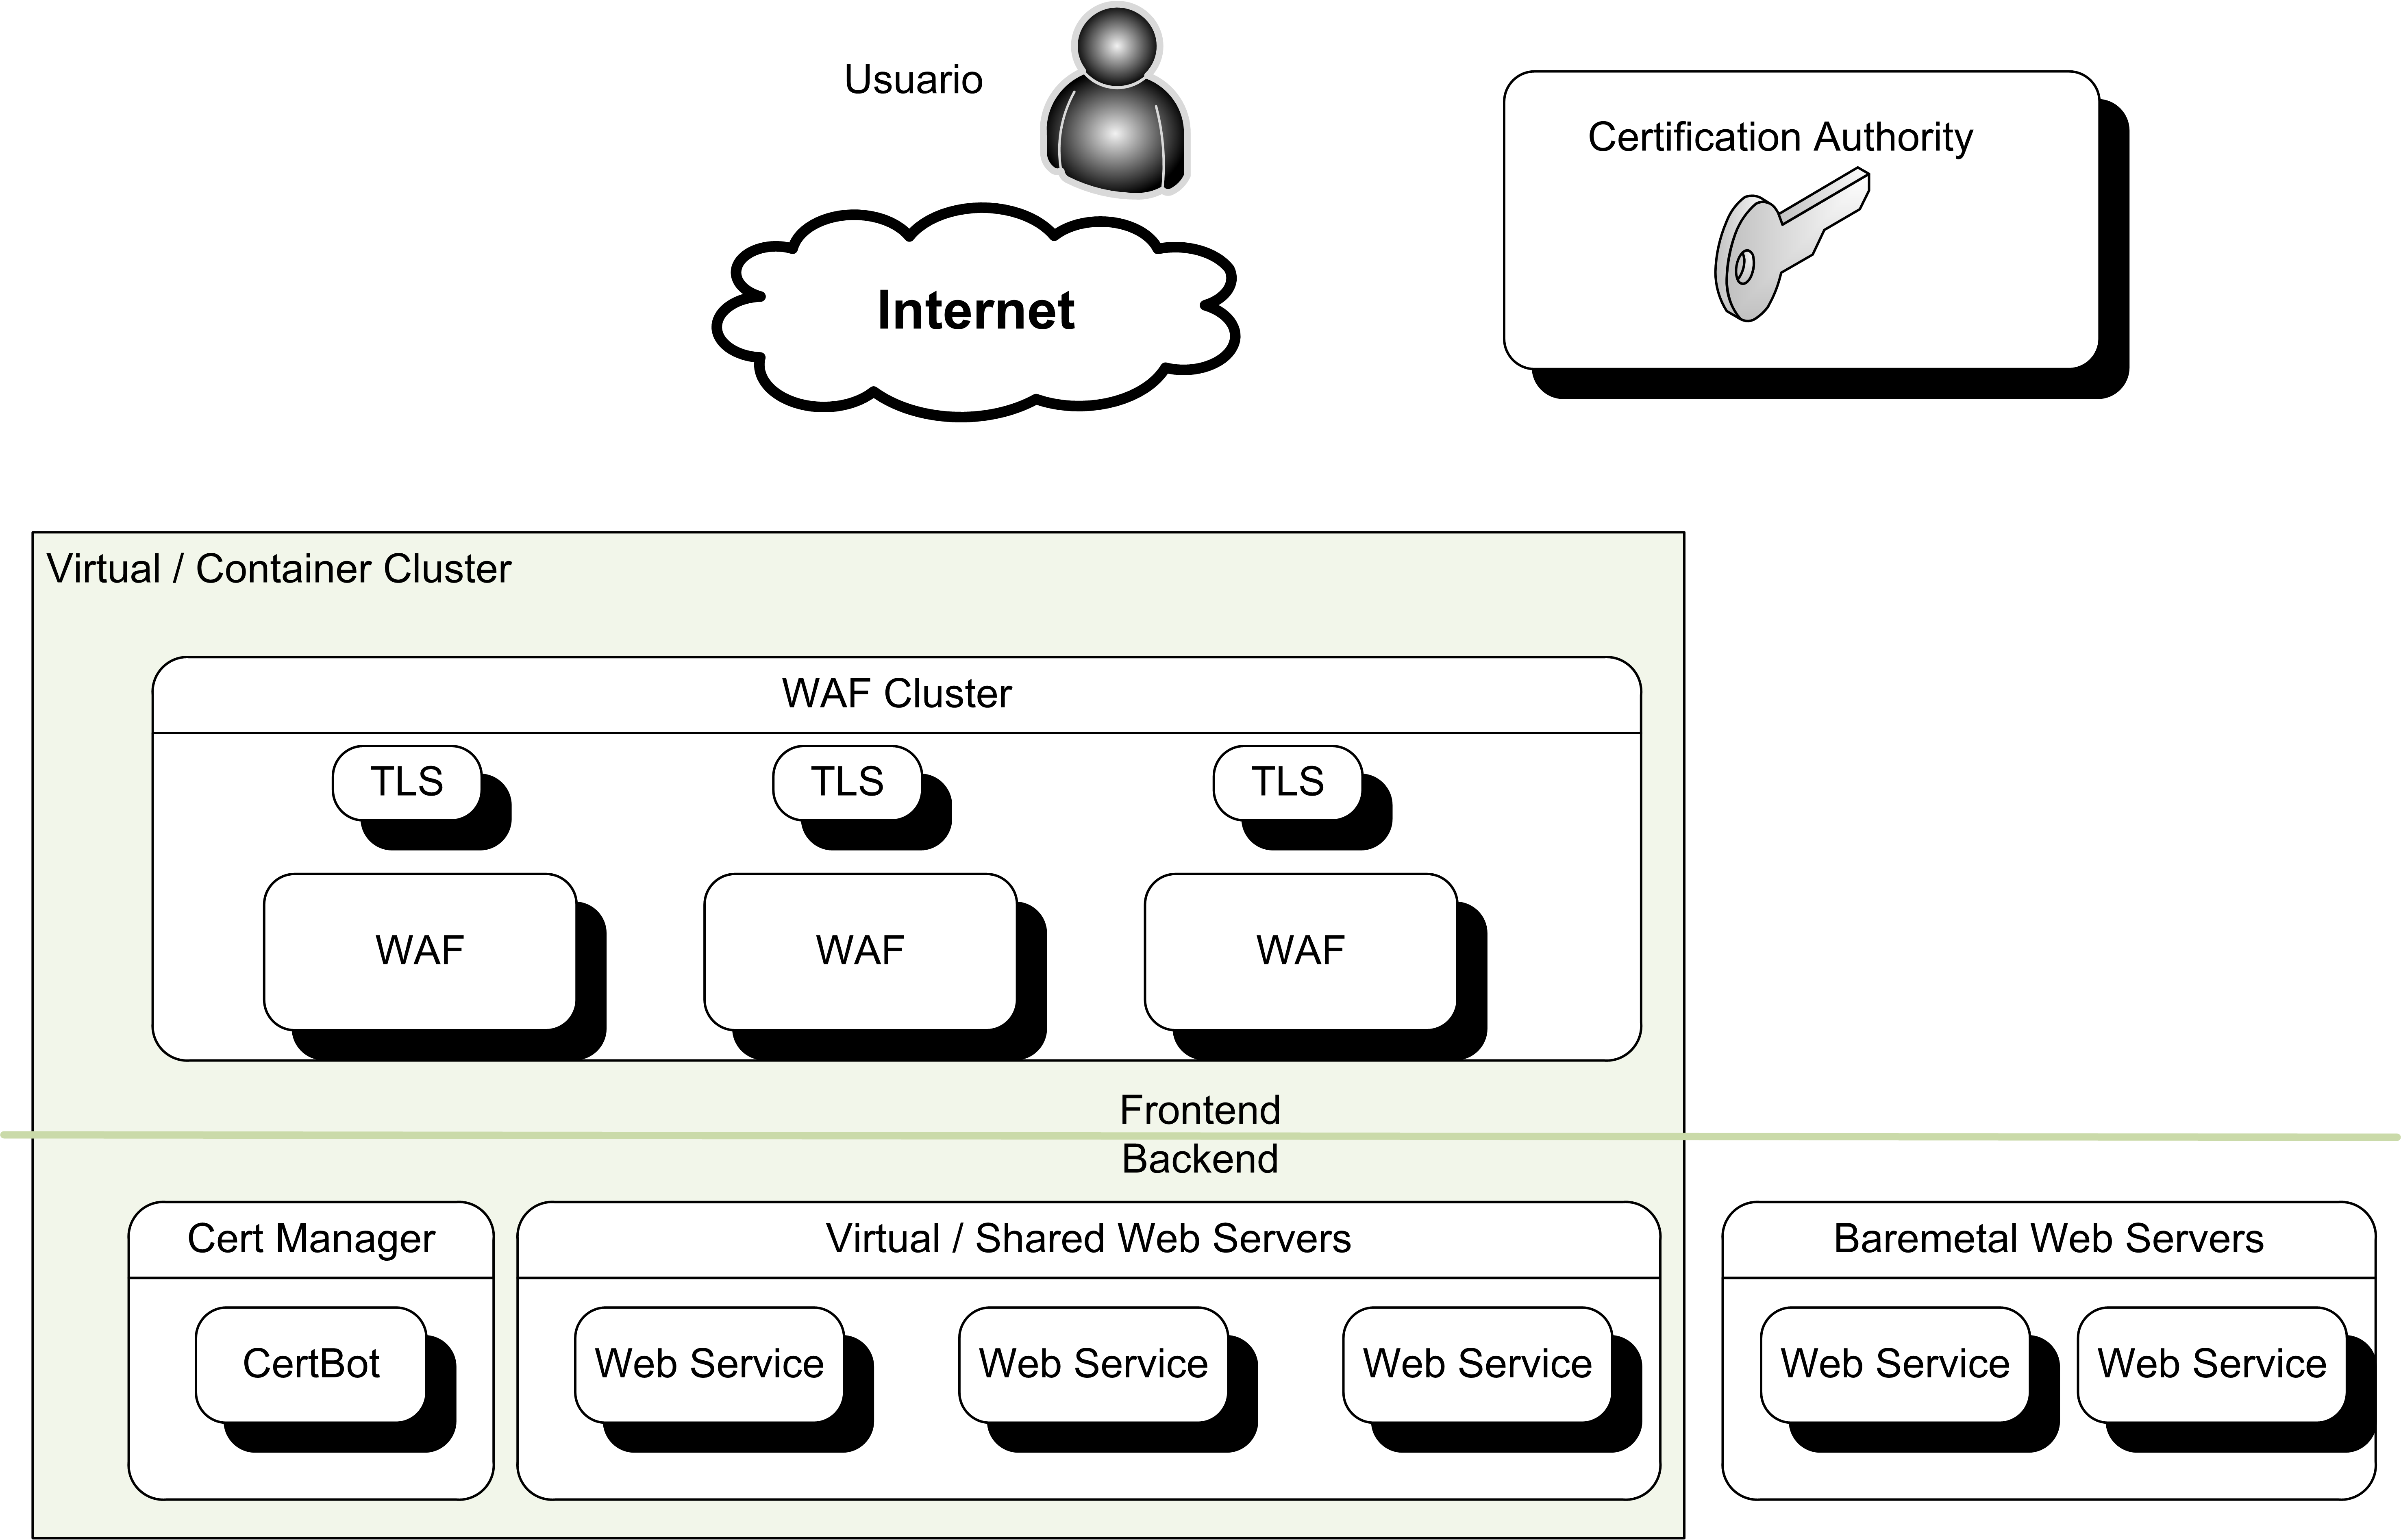
\includegraphics[width=\textwidth]{fig/Diagram_HLD}
    \caption{\small{Diseño a alto nivel de la solución}}
  \end{figure}
\end{frame}

\begin{frame}[shrink]
  \frametitle{Componentes}
  \begin{tabular}{ l c }
\usebeamertemplate***{itemize item} \acrlong{waf}.
                              & \parbox[c]{0.8\textwidth}{
\includegraphics[width=.30\textwidth,height=0.06\textheight,keepaspectratio]{fig/ModSecurityLogo}} \\ \\
\usebeamertemplate***{itemize item} Software criptográfico.
                              & \parbox[c]{0.8\textwidth}{
\includegraphics[width=.30\textwidth,height=0.06\textheight,keepaspectratio]{fig/OpenSSL_logo}} \\ \\
\usebeamertemplate***{itemize item} Virtualización (contenedores).
                              & \parbox[c]{0.8\textwidth}{
\includegraphics[width=.30\textwidth,height=0.07\textheight,keepaspectratio]{fig/DockerLogo}} \\ \\
\usebeamertemplate***{itemize item} Automatización y orquestación.
                              & \parbox[c]{0.8\textwidth}{
\includegraphics[width=.30\textwidth,height=0.07\textheight,keepaspectratio]{fig/KubernetesLogo}} \\ \\
\usebeamertemplate***{itemize item} Gestión de certificados.
                              & \parbox[c]{0.8\textwidth}{
\includegraphics[width=.30\textwidth,height=0.1\textheight,keepaspectratio]{fig/LetsEncryptLogo}} \\ \\
\usebeamertemplate***{itemize item} Políticas y controles de seguridad.
                              & \parbox[c]{0.8\textwidth}{
\includegraphics[width=.30\textwidth,height=0.15\textheight,keepaspectratio]{fig/OWASPCRSLogo}} \\ \\
    \end{tabular}
\end{frame}

\subsection{Arquitectura}
\begin{frame}[shrink]
  \frametitle{WAF. Funcionalidades}
  \begin{figure}
		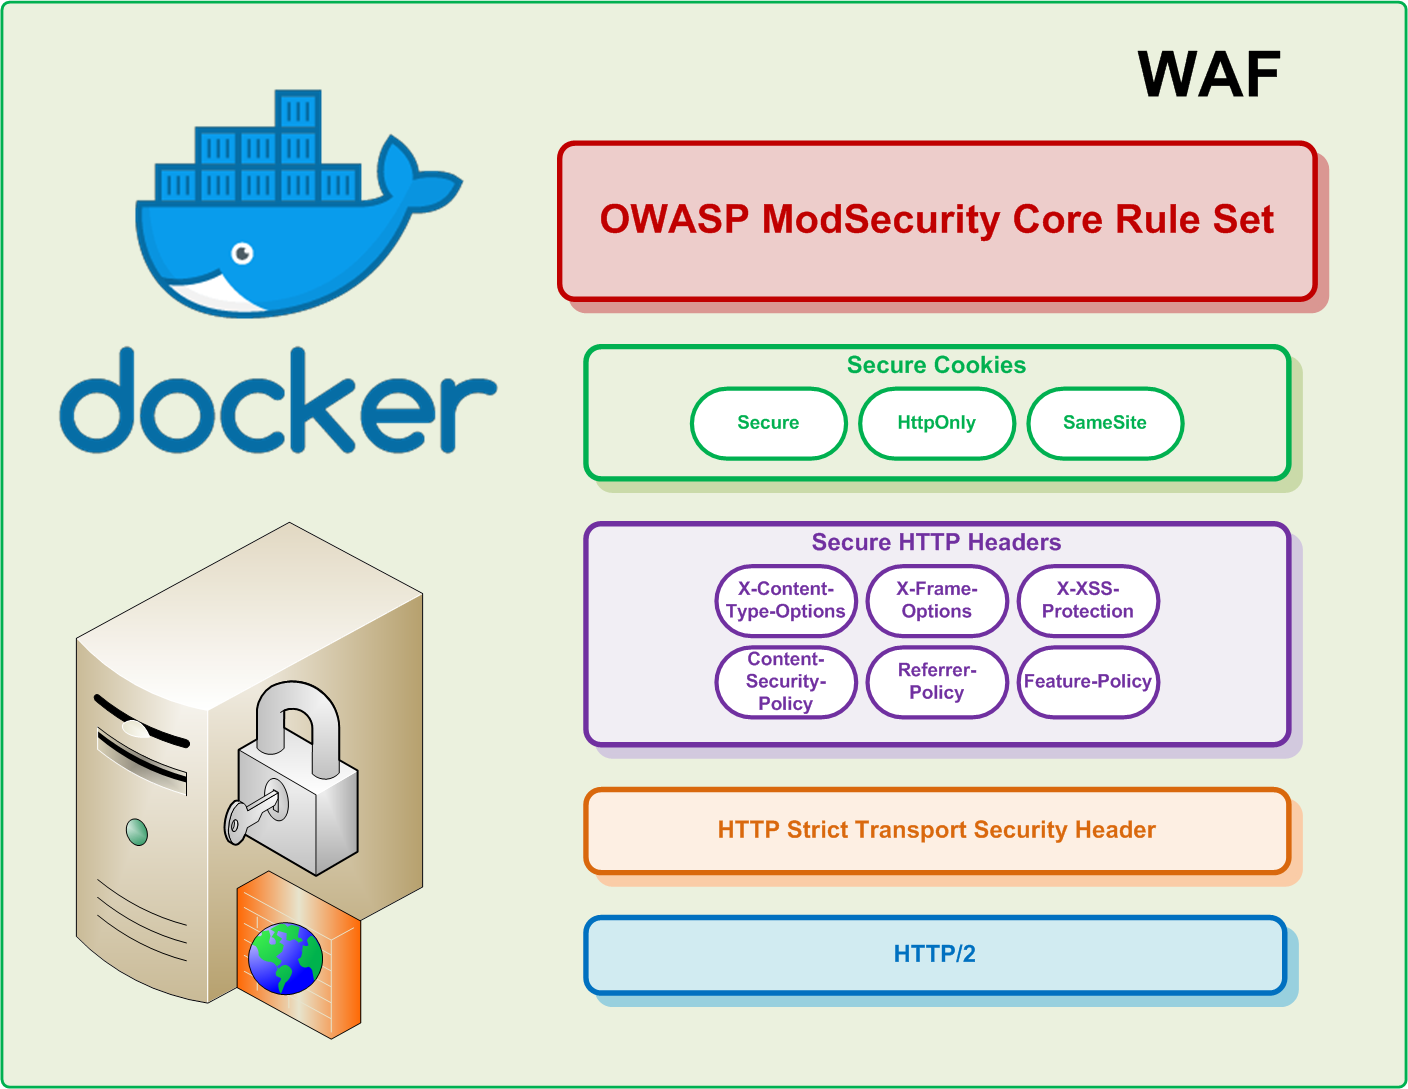
\includegraphics[width=0.9\textwidth]{fig/Diagram_Docker_WAF}
		\label{fig:Diagrama Docker WAF}
		\caption{Controles de seguridad desplegados en el contenedor Docker.}
  \end{figure}
\end{frame}

\begin{frame}[shrink]
  \frametitle{Arquitectura. Gestión de certificados}
  \begin{figure}
    \includegraphics[width=0.9\textwidth]{fig/Diagram_LetsEncypt_LLD}
    \label{fig:Diagram_LetsEncypt_LLD}
    \caption{Diagrama de comunicaciones de Let's Encrypt.}

  \end{figure}
\end{frame}

\begin{frame}[shrink]
  \frametitle{Arquitectura. Peticiones HTTP/HTTPS}
  \begin{figure}
    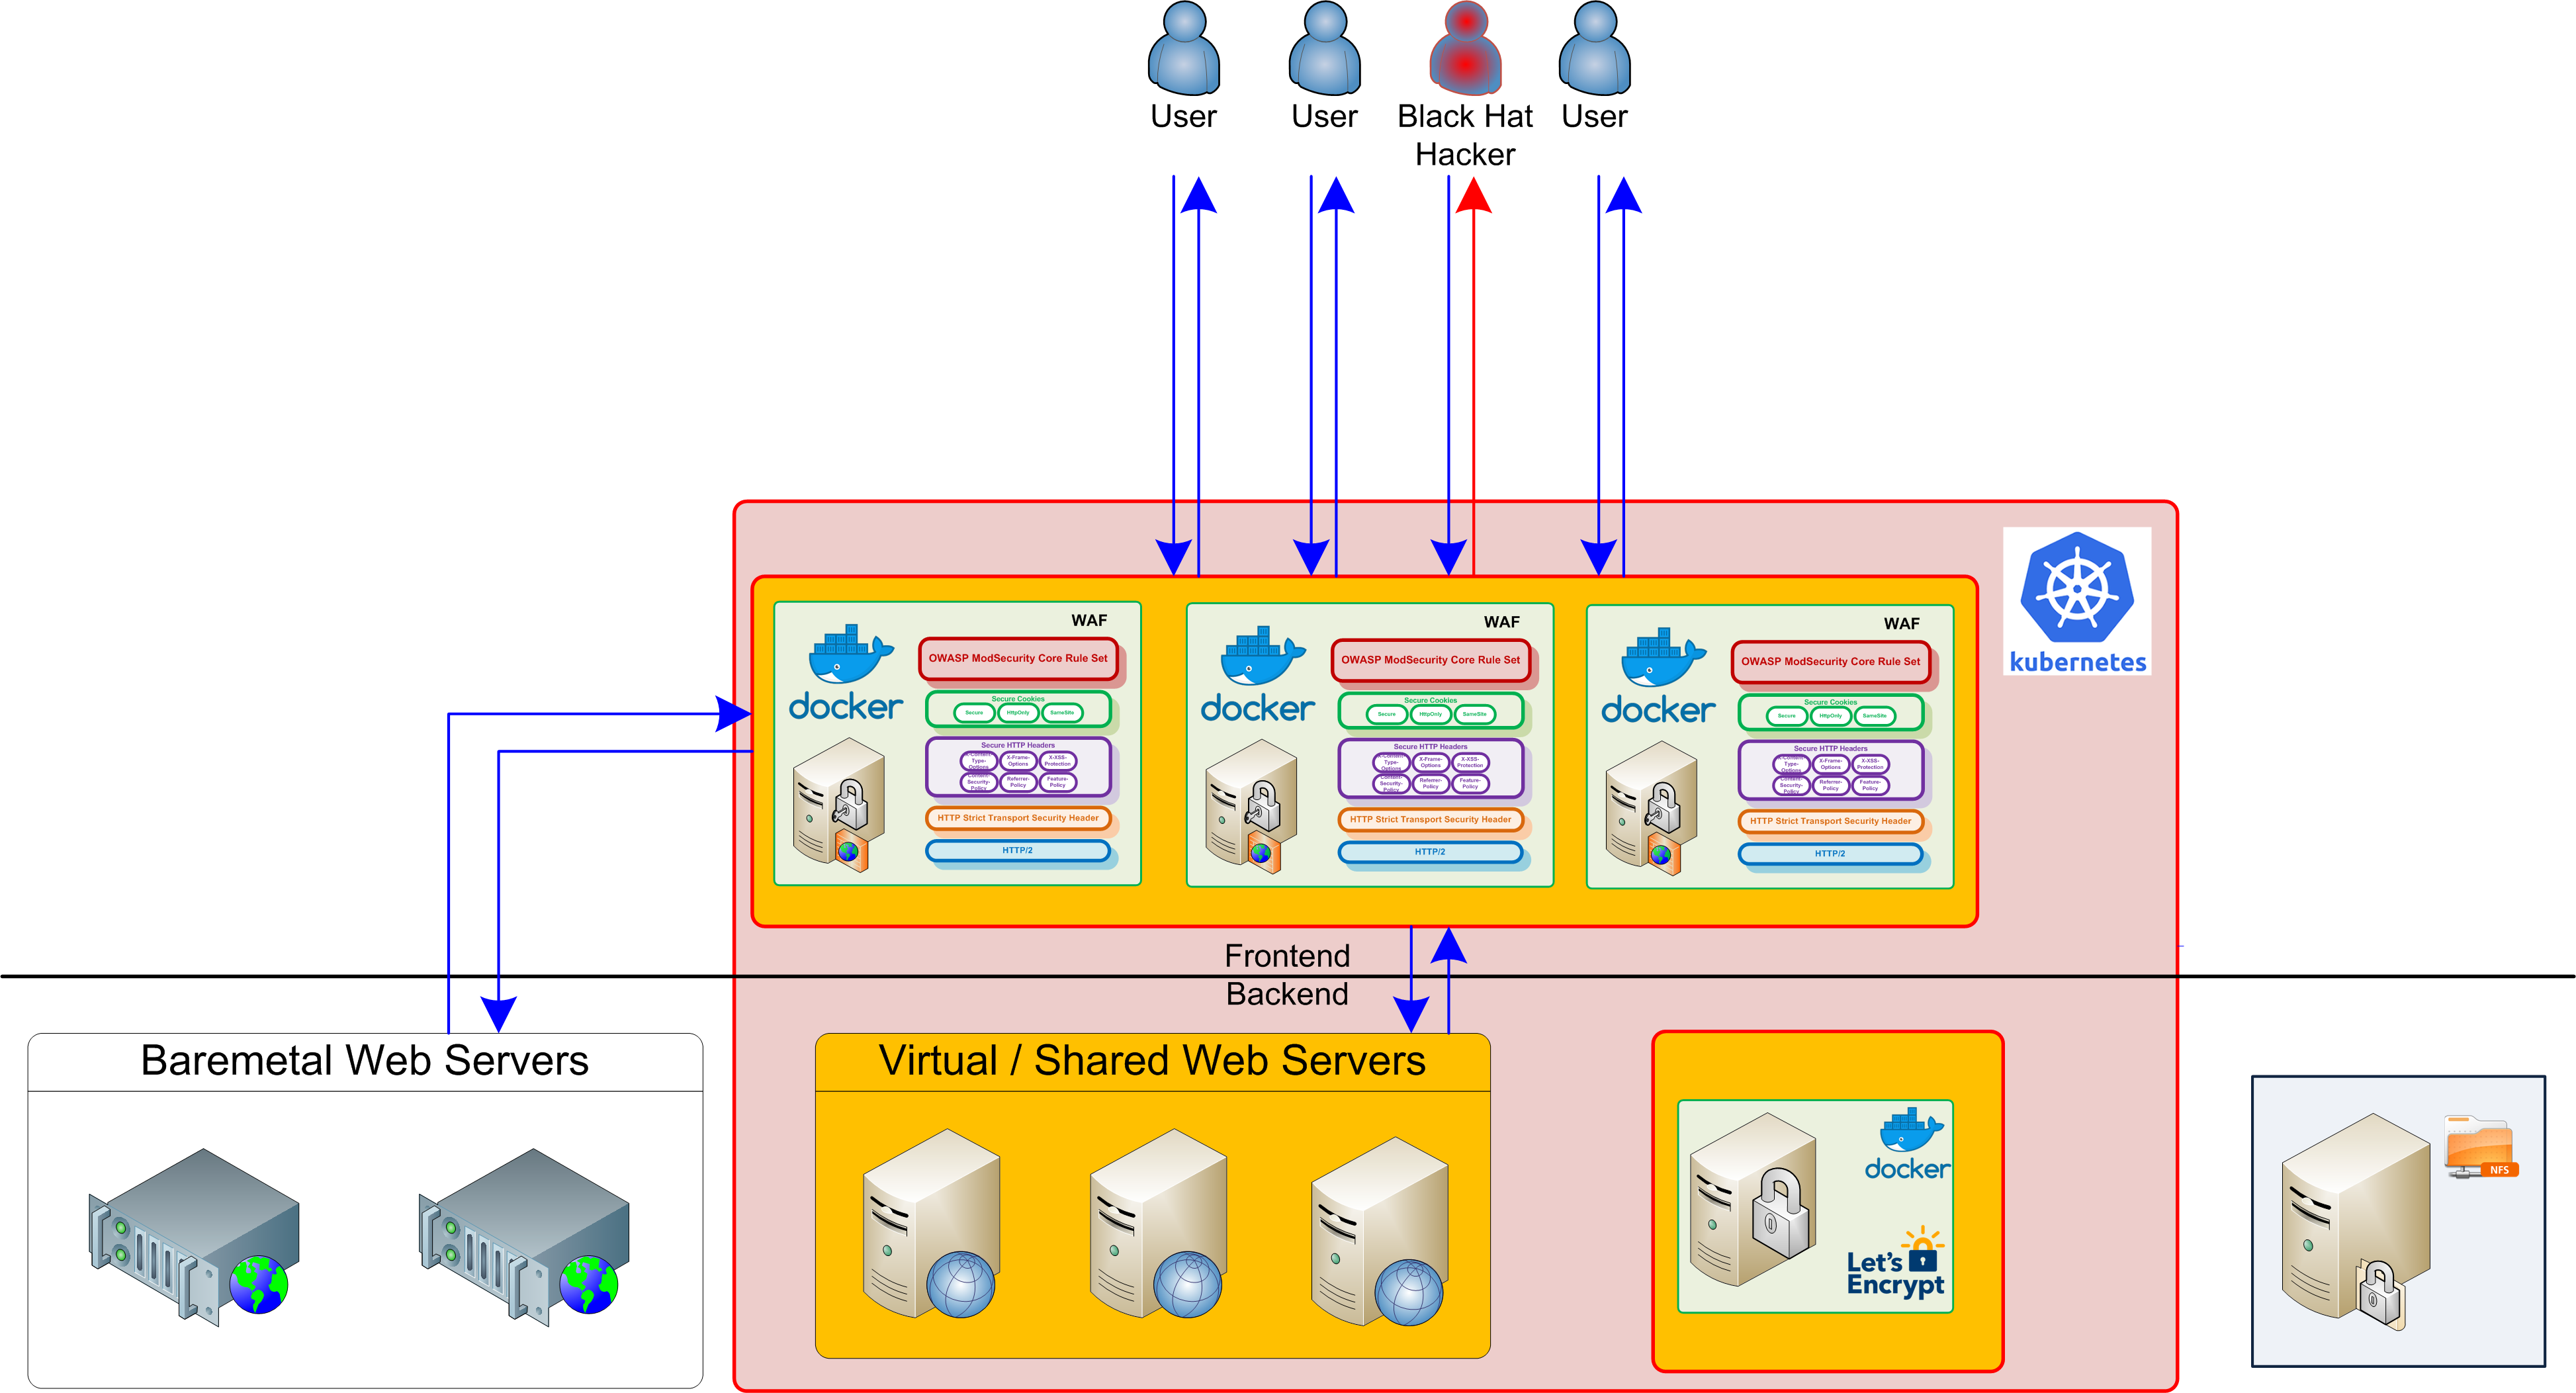
\includegraphics[width=0.9\textwidth]{fig/Diagram_HTTP_Services}
    \label{fig:Diagram_HTTP_Services}
    \caption{Peticiones HTTP/HTTPS}
  \end{figure}
\end{frame}

